% One Call is All You Need: Efficient KGQA via Question-Type-Guided Path Ranking
\documentclass[conference]{IEEEtran}

\usepackage{cite}
\usepackage{amsmath,amssymb}
\usepackage{graphicx}
\usepackage{booktabs}
\usepackage{multirow}
\usepackage{tabularx}
\usepackage{xcolor}
\usepackage{algorithm}
\usepackage{algorithmic}
\usepackage{enumitem}
\usepackage{hyperref}
\usepackage{subcaption}
\usepackage{adjustbox}
\usepackage{pifont}
\usepackage{amsthm}
\newtheorem{definition}{Definition}
\newcommand{\cmark}{\ding{51}}
\newcommand{\xmark}{\ding{55}}
\newcommand{\model}{\textsc{APR}}

\title{One LLM Call Is Enough: Adaptive Path Ranking for Efficient KGQA}

\author{\IEEEauthorblockN{Anonymous Authors}}
\begin{document}
\maketitle

\begin{center}
    \textbf{Abstract}
\end{center}
Knowledge Graph Question Answering (KGQA) aims to answer natural language questions by reasoning over structured knowledge graphs (KGs). Large Language Models (LLMs) have significantly advanced this field by acting as autonomous agents that iteratively plan and reason to navigate the graph. Current state-of-the-art methods typically employ such agentic workflows, requiring 5--10 LLM calls per query to perform planning, retrieval, and reflection. However, this multi-call paradigm suffers from high latency and computational cost, which derives in the retrieved graph structures can often be overly complex or lack the fine-grained detail necessary for precise reasoning. To address these issues, we propose \model{}, a novel framework that distills the complex reasoning process into a single-pass dense retrieval model.
Specifically, we employ a question-type classifier to predict reasoning complexity and guide candidate generation over adaptive subgraphs, followed by a late-interaction ranker with hop-aware position embeddings to identify the correct reasoning path in a single step. Experiments on WebQSP and ComplexWeb Questions demonstrate that \model{} achieves competitive accuracy compared to agentic methods while reducing LLM calls to exactly one and decreasing latency by \textbf{2--8$\times$}.
%Knowledge Graph Question Answering (KGQA) requires both semantic understanding of natural language and structured reasoning over large-scale knowledge graphs. Current state-of-the-art solutions adopt agentic Large Language Model (LLM) architectures that iteratively plan reasoning steps, retrieve subgraphs, and reflect on intermediate results through 5–10 LLM calls per query. However, this multi-call paradigm incurs prohibitive latency (1–2 seconds), suffers from cascading errors across iterations, and faces escalating API costs that fundamentally preclude real-time deployment.

\begin{IEEEkeywords}
Knowledge Graph Question Answering, Efficient Inference, Path Ranking, Question Classification
\end{IEEEkeywords}

%==============================================================================
\section{Introduction}
\begin{figure}[!t]
\centering
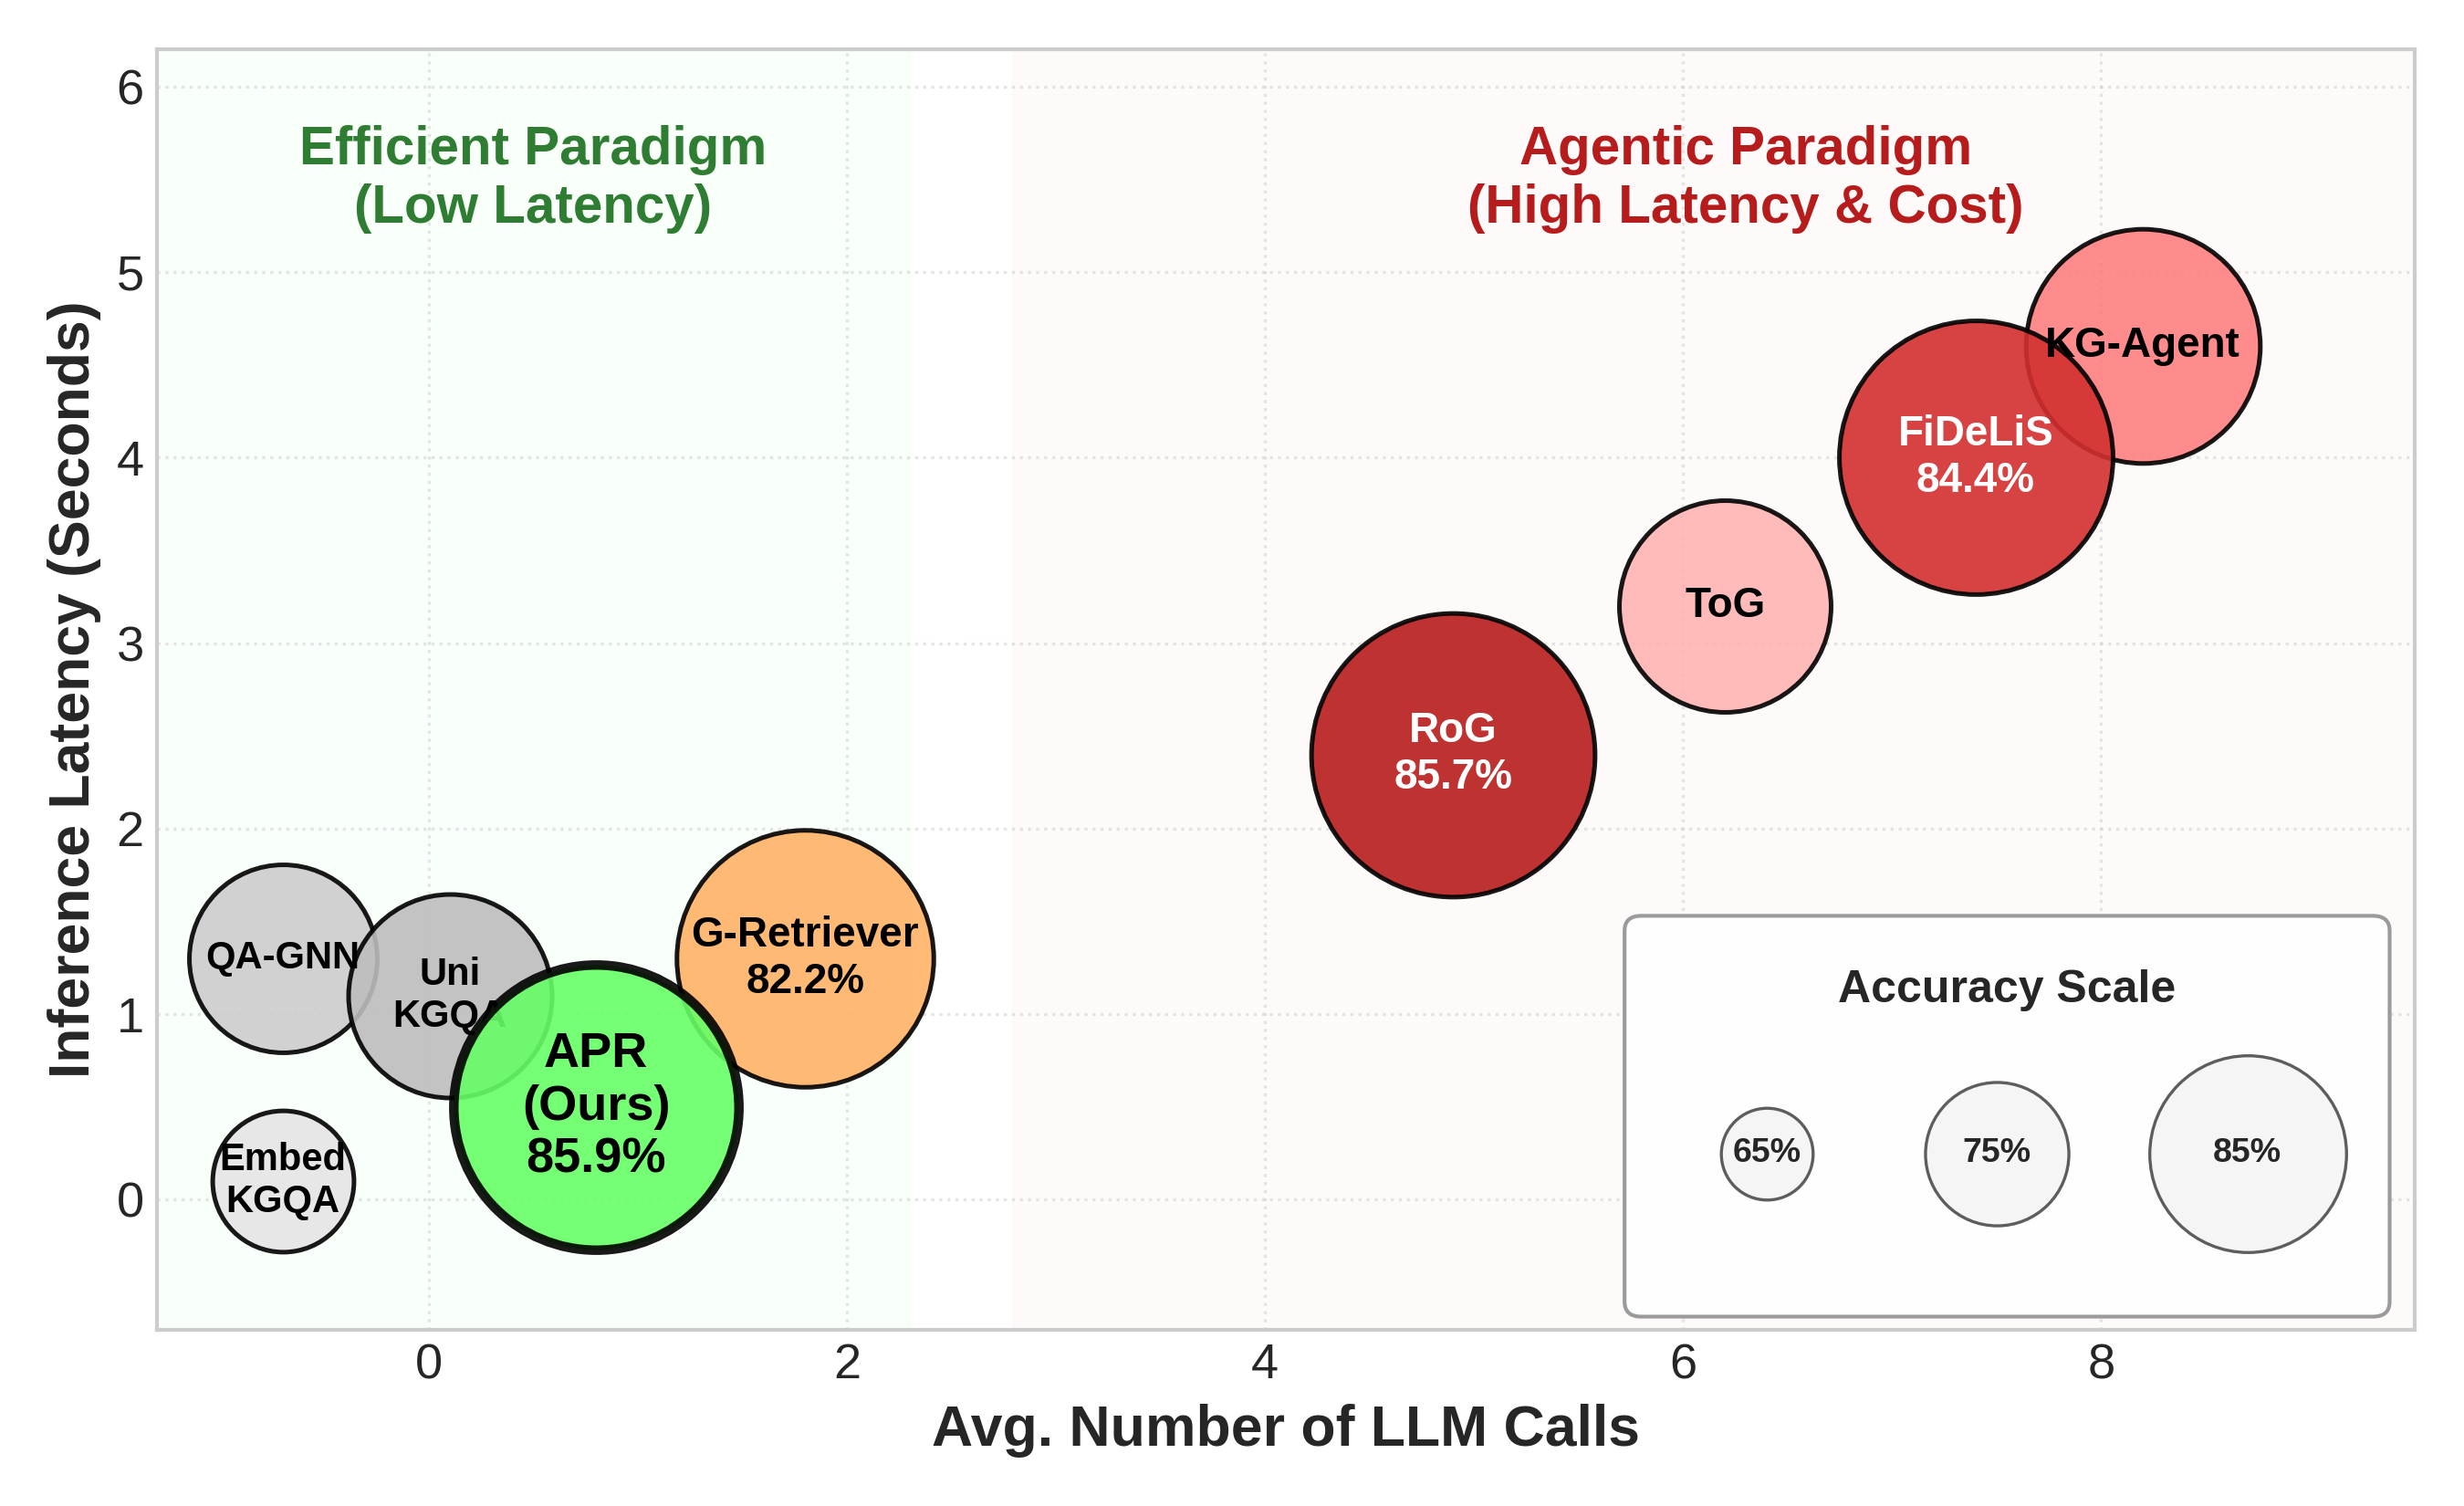
\includegraphics[width=\columnwidth,keepaspectratio,scale=1.2]{figures/figure1_tradeoff.png}
\caption{Comparison of KGQA Paradigms. The x-axis represents the number of LLM calls, the y-axis represents latency (lower is better), and the bubble size represents accuracy. \model{} (Ours) occupies the ideal “sweet spot”: high accuracy with minimal calls and low latency, contrasting with agentic methods (high cost/latency) and traditional embedding methods (lower accuracy).}
\label{fig:paradigm_bubble}
\end{figure}
%==============================================================================

Knowledge Graph Question Answering (KGQA) serves as a critical interface between human users and vast structured knowledge bases, requiring KGQA systems to understand natural language queries and perform multi-hop reasoning over graph structures \cite{ji2022kgsurvey, lan2021kbqasurvey, chakraborty2021intro}. The integration of Large Language Models (LLMs) has significantly advanced the field, enabling KGDA systems to handle increasingly complex questions with greater semantic understanding \cite{pan2024kg-llm-survey}.

Current KGQA approaches predominantly fall into three contrasting paradigms, including agentic paradigm \cite{sun2024tog, jiang2024kgagent, luo2024rog},embedding-based methods \cite{saxena2020embedkgqa, jiang2023unikgqa} and the GNN-based approaches \cite{yasunaga2021qagnn}. Unfortunately, there is an embarrassingly paradox between the Complexity and the performance. Here, a straightforward intuition is the inadequate process of the knowledge graph, leading such a paradox. For example, the agentic paradigm leans to abuse LLM to reason on a complex knowledge graph to obtain robust relation paths,  which dramatically increased time and efficiency cost. \cite{he2024gretriever} . In contrast, embedding-based methods \cite{saxena2020embedkgqa, jiang2023unikgqa} and GNN-based approaches \cite{yasunaga2021qagnn} circumvent this overhead by oversimplifying the graph structure, enabling fast, often single-call inference. Yet this simplicity severely limits semantic depth, rendering them incapable of handling complex queries that require nuanced reasoning. 

Consequently, a fundamental trade-off persists: agentic methods grapple with graph complexity through costly multi-call interactions, while embedding and GNN-based methods sacrifice expressive power for speed. The ambition for real-time, "one-call" KGQA remains elusive, as existing paradigms force an unacceptable choice between performance and efficiency. Moreover, the environmental impact of complex AI systems is a growing concern \cite{schwartz2020green, strubell2019energy}. Agentic workflows that trigger 5--10 LLM calls per query linearly multiply energy consumption. By reducing the inference process to a single LLM invocation, \model{} directly aligns with the sustainable principles of Green AI.
%Current state-of-the-art KGQA approaches predominantly follow an agentic paradigm \cite{sun2024tog, jiang2024kgagent, luo2024rog}. These methods typically operate through a sequence of steps where the LLM first decomposes the question via iterative planning and then dynamically retrieves subgraphs \cite{he2024gretriever}. While impressive, this paradigm relies on multiple sequential LLM calls (often 5--10 per query), leading to prohibitively high latency and computational costs \cite{sui2025fidelis}. Furthermore, dynamically retrieved subgraphs often contain irrelevant information, obscuring the correct reasoning path \cite{mavromatis2024gnnrag}. The ambition to achieve "one-call" KGQA is driven by the need for real-time responsiveness. Previous methods fail to achieve this: embedding-based methods \cite{saxena2020embedkgqa, jiang2023unikgqa} often lack the semantic depth to handle complex queries, while GNN-based approaches \cite{yasunaga2021qagnn} require expensive message passing. 
%如图1所示,一般会说大多数的方法,在需要好的性能的同时,存在需要多个CALL的,需要在一个复杂的图里面多次推理。于xxx,需要one call 同时保证性能, % 因为需要在一个复杂的图里面多次推理。 图过于简单,容易丢失细节。
%在这里我一般会说大多数的方法,在需要好的性能的同时,为了解决呢个问题,存在需要多个CALL的,如图1所示,,因此迫切的需要提出一种方法,去保留性能的同时减少CALL,agent 必须需要很多call 嘛？ 是不是因为需要在一个复杂的图里面多次推理。
%由于xxx,需要one call 同时保证性能, % 图过于简单,容易丢失细节。
%在这里我会加一个动机,也就是为什么这么做,比如究其本质,其需要多步的原因是因为graph不够细致,不符合问题,因此,我们由此提出了一个方法,xxx. 从而实现xxx.图1 所示。

Very Naturally, our goal is to achieving high accuracy of agentic systems with the low latency of shallow retrievers, as shown in Figure \ref{fig:paradigm_bubble}. To achive it, we are motivated to shift the reasoning burden from the LLM to a specialized, structurally-aware retriever that can adaptively otpimize the knowledge graph and identify the gold path in a single forward pass, similar to dense retrieval advances in open-domain QA \cite{karpukhin2020dpr, khattab2020colbert}.
% 受此启发,
%

% 下面这段话好像是不必要的 ,或者是重复的, 应该就是一段话介绍我们具体咋做的,


Specifically, we propose \model{}, a streamlined framework that eliminates iterative LLM calls during reasoning. \model{} utilizes a question-type classifier to guide a targeted candidate generation process, followed by a late-interaction ranker augmented with hop-aware position embeddings. The contributions of our work are list as follows:
%然后怎么做了实验,结果如何。
\begin{enumerate}
    \item we introduce a question-type guided candidate generation strategy that drastically reduces the search space by predicting reasoning complexity before path enumeration. 
    \item we develop a hop-aware late interaction ranker that captures structural alignment between questions and relation paths without requiring iterative generation. \item we demonstrate through extensive experiments that \model{} achieves state-of-the-art performance on WebQSP and CWQ while offering a \textbf{2--8$\times$} speedup over agentic baselines.
\end{enumerate}




%==============================================================================
\section{Related Work}
%==============================================================================

\subsection{Knowledge Graph Question Answering}

KGQA methods have evolved through several distinct paradigms. \textbf{Semantic parsing} approaches \cite{yih2016webqsp, yu2018spider, lei2024spider2} translate questions into executable logical forms over a knowledge base. While precise when successful, these methods are sensitive to linguistic variation and require extensive grammar engineering, limiting their applicability to open-domain questions with diverse surface forms.

\textbf{Embedding-based} methods learn joint representations of questions and graph structures. UniKGQA \cite{jiang2023unikgqa} unifies retrieval and reasoning through a shared pre-training objective, while ReaRev \cite{luo2022rearev} introduces adaptive reasoning through iterative refinement of entity representations. GNN-based approaches \cite{yasunaga2021qagnn} propagate question semantics through retrieved subgraphs via message passing. These methods avoid explicit logical form generation but often require expensive online graph operations, and their fixed-vector representations struggle to capture fine-grained semantic alignments between question phrases and specific relations.

The \textbf{agentic paradigm} emerged with methods like Think-on-Graph (ToG) \cite{sun2024tog}, which frames the LLM as an autonomous agent performing beam search over the KG. In ToG, the LLM is invoked at every hop to evaluate neighbors and select the most promising paths, often requiring dozens of calls for deep reasoning. Subsequent work has sought to optimize this process: KG-Agent \cite{jiang2024kgagent} introduces an explicit planning phase where the LLM drafts a reasoning skeleton before navigating the graph, reducing redundant exploration. RoG \cite{luo2024rog} emphasizes a "plan-then-retrieve" approach, generating candidate relation paths as a plan and then grounding them in the graph, which decouples reasoning from retrieval. FiDeLiS \cite{sui2025fidelis} introduces deductive scoring for stepwise verification of intermediate results. While these methods achieve high accuracy by leveraging LLM reasoning at inference time, they fundamentally rely on multiple sequential LLM calls (typically 5--10), leading to latencies of several seconds per query. This motivates the search for architectures that can achieve comparable accuracy with fewer LLM invocations.

\subsection{Retrieval and Efficient Matching}

To reduce reliance on multi-step LLM inference in agentic KGQA systems, recent work has explored shifting reasoning complexity from online generation to retrieval and matching. Retrieval-Augmented Generation (RAG) \cite{lewis2020rag}, which traditionally retrieves unstructured text to condition LLM generation, presents a natural opportunity in the KG setting: structured graph evidence can serve as precise grounding context, allowing much of the reasoning to be resolved during retrieval rather than generation. At the same time, adapting RAG to KGs introduces new challenges: naive linearization of subgraphs \cite{pan2024kg-llm-survey} often results in "context contamination" where the LLM struggles to discern relevant connections amidst graph noise. GNN-RAG \cite{mavromatis2024gnnrag} addresses this by using Graph Neural Networks to score graph neighbors, but still requires expensive online message passing. These approaches highlight the importance of retrieving \emph{precise, structured} context rather than noisy subgraphs---a principle that motivates path-based retrieval where the retrieval unit is a semantic reasoning path rather than a document or node set.

Designing such path-based retrieval mechanisms inevitably raises trade-offs between accuracy and efficiency, which has been well-studied in open-domain QA \cite{gao2021densesurvey}. Dense retrieval methods \cite{karpukhin2020dpr, izacard2022contriever} replace keyword matching with learned embeddings, enabling semantic matching but compressing all information into fixed-size vectors. Late interaction models like ColBERT \cite{khattab2020colbert, santhanam2022colbertv2} preserve token-level information while allowing offline document encoding, achieving a more favorable balance between precision and latency. This token-level matching paradigm is particularly appealing for KGQA, where subtle lexical cues in the question (e.g., “capital of the country”) must align with specific relations in the path (e.g., “country.capital”).

Prior work has also recognized that KGQA questions vary substantially in reasoning complexity \cite{gu2021beyond, cao2022kqa}. Some questions require single relation traversal; while others demand multi-hop reasoning or involve additional constraints, such as aggregation or numeric computation. Existing systems handle this variation implicitly through beam search depth or agent iteration limits, but explicit complexity prediction could enable more targeted candidate generation and reduce wasted computation on simple queries.

\section{Methodology}
\label{sec:methodology}

A central challenge in KGQA is retaining the reasoning fidelity of agentic methods without incurring the high latency and cost of multi-step LLM interaction. To this end, we introduce \model{}, a framework that replaces iterative LLM-driven exploration with adaptive, structurally aware path ranking. 

Given a natural language query $q$, APR initially anchors it to a topic entity $e_{topic}$ via entity linking. The system then estimates the reasoning complexity of $q$ by predicting the appropriate hop range required for answering the question, which directly constrains subsequent graph exploration (\textbf{Question-Type Classification}). Guided by this prediction, candidate relation paths are enumerated from $e_{topic}$ using a constrained Breadth-First Search (BFS) up to a maximum depth $h_{max}$, while paths inconsistent with the predicted hop range are pruned early (\textbf{Guided Candidate Generation}). All surviving candidate paths are next evaluated in parallel by a late-interaction ranker that performs fine-grained token-level alignment between the question and each path (\textbf{Late-Interaction Path Ranking}). The top ranked paths are retained, their corresponding answer entities retrieved, and this structured evidence is finally provided to a Large Language Model (LLM) exactly once to synthesize the final natural language answer (\textbf{Answer Synthesis}). The complete inference procedure is summarized in Algorithm~\ref{alg:inference} and illustrated in Figure~\ref{fig:architecture}.


%Our proposed strategy differs sharply from previous approaches. Agentic KGQA systems are characterized by their reliance on repeated LLM invocations to plan, expand neighbors, and verify intermediate steps \cite{sun2024tog, jiang2024kgagent, luo2024rog}. While this affords flexibility, it inextricably couples accuracy with a high volume of sequential calls, causing latency and cost to balloon as hop depth increases. In contrast, \model{} amortizes the reasoning burden into a supervised ranker: once candidate paths are generated, scoring becomes a parallelizable operation devoid of iterative generation. Unlike generate-then-retrieve architectures that still depend on multi-step prompting \cite{jiang2023structgpt, luo2024chatkbqa}, we embed structural awareness directly into the retrieval model itself via hop-aware supervision. Finally, distinct from one-call baselines that rely primarily on prompting strategies \cite{zhang2024trustuqa, ao2025lightprof}, \model{} explicitly learns a late-interaction operational matching over KG paths---a critical capability when subtle lexical cues must be aligned with specific relations.


\subsection{Problem Formulation}

Knowledge Graph Question Answering (KGQA) requires mapping a natural language question to a sequence of relations in a knowledge graph that leads from a topic entity to the correct answer. While prior methods often perform this reasoning through iterative graph exploration guided by an LLM, we instead formulate KGQA as a path discrimination problem. Any KGQA instance can be viewed as identifying a correct reasoning path from a topic entity to an answer entity. We therefore first formalize the general KGQA task and then present its reformulation as a path discrimination problem.

\begin{definition}[]
\textbf{KGQA} aims to answer natural language questions by leveraging a knowledge graph $\mathcal{G}=(\mathcal{E}, \mathcal{R})$ as context for answers retrieval, where each fact is a triple $(e, r, e')$, representing a directed connection from a head entity $e$ to a tail entity $e'$ via a relation $r$. Given a question $q$ and a topic entity $e \in \mathcal{E}$ identified from $q$, the objective of KGQA is to identify the answer entity(s) $e' \in \mathcal{E}$ such that correctly satisfy the information requested by $q$ with respect to $\mathcal{G}$.
\end{definition}

% This challenge can be formulated as a \textbf{path discrimination} problem. Let $\mathcal{P}_e$ denote the set of all valid relation paths originating from $e$, where a path $p \in \mathcal{P}_e$ is defined as a sequence of relations $p = (r_1, r_2, \dots, r_h)$ of length $h$ (number of hops), bounded by a maximum depth $h_{\max}$ (e.g., $h_{\max}=4$ for CWQ and WebQSP datasets). Instead of employing agentic systems that construct paths iteratively through sequential decision-making, we learn a scoring function $f_{\text{rank}}(q, p)$ to rank a pre-enumerated set of candidate paths. The objective is to assign higher scores to paths that terminate at entities relevant to the correct answer for $q$, thereby facilitating effective retrieval of precise context.
% We define a Knowledge Graph $\mathcal{G} = (\mathcal{E}, \mathcal{R}, \mathcal{T})$ as a collection of entities $\mathcal{E}$ and relations $\mathcal{R}$, engaged in a set of facts $\mathcal{T}$. Each fact is a triple $(e, r, e')$, representing a directed connection from a head entity $e$ to a tail entity $e'$ via a relation $r$.
% Given a question $q$, which we link to a primary topic entity $e$, our goal is to identify the correct answer entities $\mathcal{A} \subset \mathcal{E}$. These answers are the destination of a valid reasoning path $p$ that's from $e$.


% Knowledge Graph Question Answering (KGQA) demands navigating the complex structure of a Knowledge Graph (KG) to discover facts that satisfy a user's question or intent. The difficulty is not just about retrieving these facts, but also about converting semantics of human language into precise structural traversals.

% We define a Knowledge Graph $\mathcal{G} = (\mathcal{E}, \mathcal{R}, \mathcal{T})$ as a collection of entities $\mathcal{E}$ and relations $\mathcal{R}$, engaged in a set of facts $\mathcal{T}$. Each fact is a triple $(e, r, e')$, representing a directed connection from a head entity $e$ to a tail entity $e'$ via a relation $r$.
% Given a question $q$, which we link to a primary topic entity $e$, our goal is to identify the correct answer entities $\mathcal{A} \subset \mathcal{E}$. These answers are the destination of a valid reasoning path $p$ that's from $e$.

\begin{definition}
\textbf{Path Discrimination Reformulation}. Let $\mathcal{P}_e$ denote the set of all valid relation paths originated from $e$. Each path $p \in \mathcal{P}_e$ is defined as a sequence of relations $p = (r_1, r_2, \dots, r_{h(p)})$, where $h(p)$ denotes the length of the path (i.e., the number of hops) and is bounded by a lower and an upper limit (i.e., $h_{p,min} \leq h(p) \leq h_{p,max}$).  Traversing a path $p$ from $e$ leads to one or more entities $e'$ in the graph. The task is to learn a ranking function $f_{rank}(q, p)$ that assigns higher probabilities to paths that are semantically aligned with the question $q$ and lead to the correct answer entities $e'$ and rank them from high to low. 
\end{definition}

In this work, we consider a global maximum hop limit of $h_{p,max} \leq 4$, for all paths $p$, consistent with the CWQ and WebQSP benchmarks.

\begin{figure*}[!t]
\centering
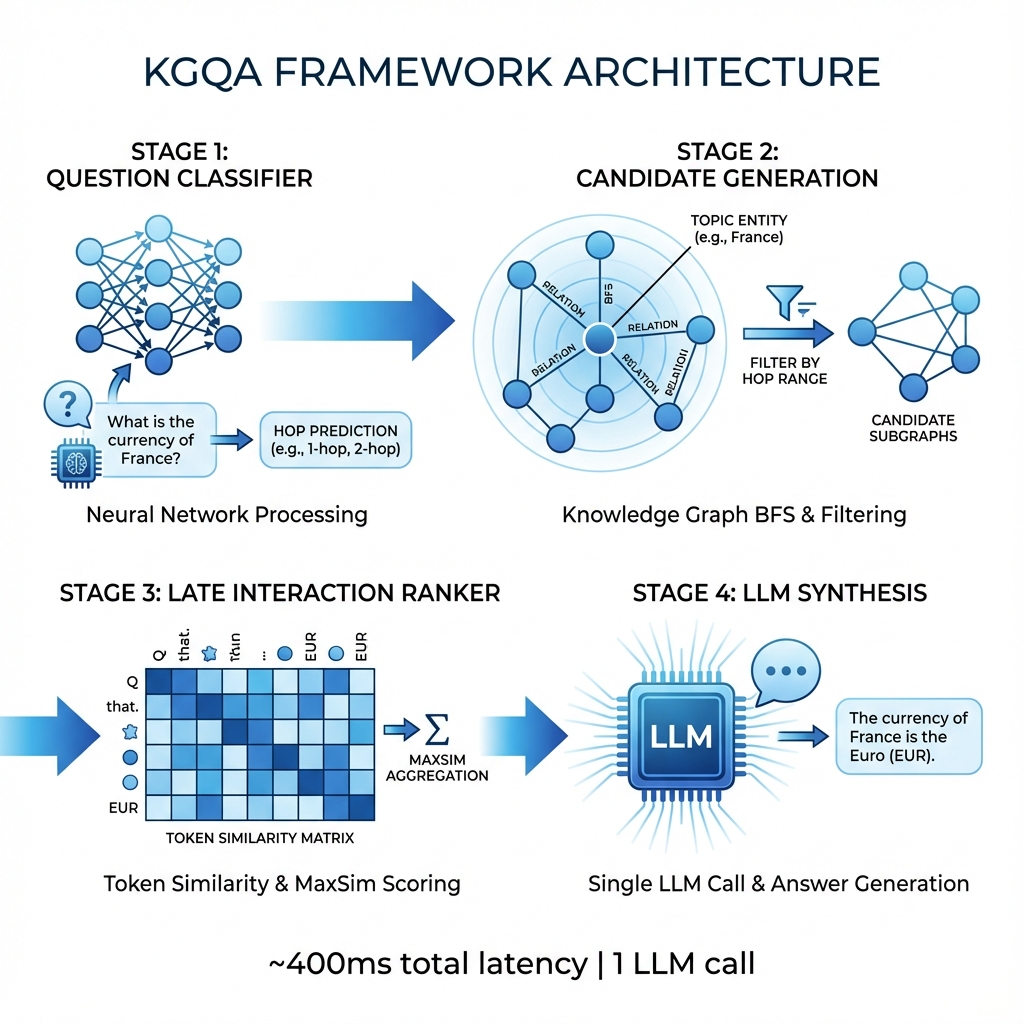
\includegraphics[width=\textwidth,keepaspectratio]{figures/MethodArc.png}
\caption{System architecture of \model{}. \textbf{Stage 1}: Question-type classifier predicts reasoning complexity. \textbf{Stage 2}: Constrained BFS generates candidate paths. \textbf{Stage 3}: Late interaction ranker scores all candidates in a single forward pass. \textbf{Stage 4}: Top-ranked paths are fed to LLM for final answer synthesis---the only LLM invocation.}
\label{fig:architecture}
\end{figure*}

\begin{algorithm}[t]
\caption{\model{} inference (classifier-guided filtering)}
\label{alg:inference}
\begin{algorithmic}[1]
\REQUIRE Question $q$, Max Hops $h_{max}$, Top-$n$ threshold $N_{top}$
\ENSURE Answer string $\hat{a}$
\STATE $e \leftarrow \textsc{TopicEntityLinking}(q)$
\STATE $\mathcal{P} \leftarrow \textsc{BFSPaths}(e, h_{max})$ \ref{sec:methodology}
\STATE $(h_{min}, h_{proc}) \leftarrow f_{cls}(q)$ \COMMENT{Predict complexity range} \ref{eq:type_prediction}
\STATE $\mathcal{P}_{e}' \leftarrow \{p \in \mathcal{P} : h_{min} \le h(p) \le h_{proc}\}$ \ref{eq:PePrime}
\STATE $S_{scores} \leftarrow f_{rank}(q, \mathcal{P}_{e}')$ \COMMENT{Batched MaxSim} \ref{eq:maxsim}
\STATE $\mathcal{P}_{top} \leftarrow \textsc{SelectTopN}(\mathcal{P}_{e}', S_{scores}, N_{top})$ \ref{eq:maxsim}
\STATE $c \leftarrow \{(p, \textsc{Traverse}(p)) \mid p \in \mathcal{P}_{top}\}$ \ref{sec:methodology}
\STATE $\hat{a} \leftarrow \textsc{LLMGen}(q, c)$
\RETURN $\hat{a}$ \ref{sec:methodology}
\end{algorithmic}
\end{algorithm}

\subsection{Question-Type Classification}
Existing KGQA systems, including agentic methods \cite{jiang2024kgagent,luo2024rog,tan2025pog}, have long recognized that questions vary in reasoning complexity and often distinguished by hop count. For instance, a question such as “Who directed Inception?” requires only one-hop traversal, whereas “What is the nationality of the spouse of Tom Hanks?” requires chaining multiple relations. Nevertheless, these methods typically incorporate such distinctions implicitly during online LLM-driven reasoning, for example by adjusting exploration depth, beam width, or planning steps at inference time, rather than using them to proactively constrain the search space. 

Moreover, question reasoning complexity is not limited to hop-based patterns; additional forms of variation arise in practice. In particular, numeric questions impose an orthogonal constraint: rather than identifying a single target entity, they require aggregation over a set of retrieved entities or literals. For example, answering “How many children does Tom Hanks have?” involves enumerating all child entities and computing their cardinality, regardless of whether the underlying relational structure is shallow or deep. As a result, treating numeric questions solely as one-hop or multi-hop entity queries leads to unnecessary candidate expansion and ineffective retrieval.

Motivated by these observations, we characterize reasoning complexity along two orthogonal dimensions: \textit{structural depth} (one-hop vs. multi-hop) and \textit{answer modality} (relational entity vs. numeric aggregation). This formulation yields a four-class taxonomy, with each class associated with a specific hop range, as summarized below. We then train a multi-label classifier to predict question type with the required hop range and answer modality, enabling downstream components to restrict candidate generation and avoid exploring irrelevant graph structure.

\noindent \textit{Question-type Taxonomy}: 
% \textbf{One-hop Non-numeric} questions are answerable via a single direct relation lookup, such as asking for a movie's director. \textbf{Multi-hop Non-numeric} questions require a chain of 2--4 relations to locate the answer entity, for instance querying the nationality of someone's spouse. \textbf{One-hop Numeric} questions require aggregation over immediate neighbors, such as counting someone's children or retrieving a literal like height. Finally, \textbf{Multi-hop Numeric} questions demand multi-step traversal followed by aggregation, such as counting how many awards a director has won.
\begin{itemize}
    \item \textbf{1-Hop Non-Numeric}: Direct relation lookups requiring at most one relational travsal (1 hop).
    \item \textbf{Multi-Hop Non-Numeric}: Compositional reasoning involving chains of multiple relations. (2-4 hops)
    \item \textbf{1-Hop Numeric}: Aggregations over immediate neighbors. (1-2 hops)
    \item \textbf{Multi-Hop Numeric}: Multi-step relational traversals followed by numeric aggregation. (2-4 hops)
\end{itemize}

For question-type classification, we adopt a SentenceTransformer-based encoder to obtain a fixed-dimensional representation of the question. The encoded representation is passed to a lightweight MLP classifier to predict the question type. For clarity, we briefly summarize the classification logic in Eq. (1).

\begin{equation}
    \hat{t} = \arg\max\!\Big(\text{Softmax}\big(\text{MLP}(\text{Pool}(f_{enc}(q)))\big)\Big)
    \label{eq:type_prediction}
\end{equation}

\noindent where, $\hat{t}$ denotes the predicted question type of the question $q$, selected via the $\arg\max$ operator; $f_{enc}$ is a SentenceTransformer-based text encoder that maps $q$ to contextualized token representations; $\text{Pool}(\cdot)$ denotes a pooling operation that aggregates token representations into a fixed-dimensional vector (e.g., using the [CLS] token); $\text{MLP}(\cdot)$ is a multi-layer perceptron that maps the pooled representation to a vector of class logits; and $\text{Softmax}(\cdot)$ converts logits into a probability distribution over the predefined question-type 

%The predicted type $\hat{t}$ imposes strict constraints on the subsequent search: for instance, predicting ``1-Hop'' allows us to discard all multi-hop candidates immediately, reducing the search space by up to 86\% (Table~\ref{tab:classifier}).


\begin{table}[t]
\centering
\caption{Candidate reduction achieved by question-type classification. The 4-class taxonomy enables aggressive pruning, especially for one-hop queries.}
\label{tab:classifier}
\begin{tabular}{lcc}
\toprule
Type & Avg Candidates & Reduction \\
\midrule
One-hop (Ent) & 21 & 84\% \\
Multi-hop (Ent) & 192 & 38\% \\
One-hop (Num) & 18 & 86\% \\
Multi-hop (Num) & 145 & 51\% \\
\bottomrule
\end{tabular}
\end{table}

\subsection{Candidate Path Generation}

Given the predicted reasoning complexity, we enumerate candidate relation paths in this stage using a constrained Breadth-First Search (BFS). In particular, based on the predicted question type $\hat{t}$ and its topic entity $e$, we apply the corresponding hop range $[h_{\hat{t},min}, h_{\hat{t},max}] $ to prune generated paths, resulting in a pruned path set $\mathcal{P}_{e}'$ that contains only those whose lengths fall within the predicted range. 

\begin{equation}
    \mathcal{P}_{e}' = \{ p \in \textsc{BFS}(e) \mid h_{p,min} \le h(p) \le h_{p,max} \}
    \label{eq:PePrime}
\end{equation}

\subsection{Late Interaction Path Ranking}

To identify paths that best support the answer, we further rank all paths in the pruned candidate path set by scoring them against the question for relevance. Traditional bi-encoders compress the entire input into a single vector and they sometimes fail to capture fine-grained alignments \cite{karpukhin2020dpr}. For example, the phrase ``capital of'' in a question must specifically align with the relation `\texttt{location.country.capital}`, which might be neglected in pooled global representations. To rectify this, we adapt \textbf{Late Interaction}, as depicted in Figure~\ref{fig:late-interaction}, to preserve token-level fidelity and enable precise, "soft" alignment between query terms and graphical relations. More importantly, we introduce hop-aware path embeddings that explicitly encode a relation’s position within a reasoning chain, and design depth-aware training objectives that supervise both intermediate hops and final path ranking. Together, these components ensure that structurally valid reasoning paths are ranked accurately, enabling reliable retrieval of answer-supporting evidence from the pruned candidate set.

\begin{figure}[t]
    \centering
    \includegraphics[width=0.9\linewidth]{figures/Figure_LateInteraction.png}
    \caption{Overview of the proposed Late Interaction method for preserving token-level information and enabling fine-grained, soft alignment between question tokens and candidate paths.}
    \label{fig:late-interaction}
\end{figure}

\subsubsection{Token Encoding}
Both the question $q$ and each candidate path $p$ are first encoded by the transformer $f_{enc}$. We project the resulting contextualized representations to a lower-dimension to optimize meaningful comparison:
\begin{align}
    \mathbf{Z}_{q} &= \text{Proj}(f_{enc}(q)) \\
    \mathbf{Z}_{p} &= \text{Proj}(f_{enc}(p))
\end{align}
\noindent where $\mathbf{Z}_{q} \in \mathbb{R}^{L_q \times d_{proj}}$ and $\mathbf{Z}_{p} \in \mathbb{R}^{L_p \times d_{proj}}$ denote the token-level embeddings of the question and the corresponding candidate path, respectively, with $L_q$ and $L_p$ representing their token counts;  $d_{proj}$ is the size of the projected embedding space (e.g., 128 being used in this paper); and $\text{Proj}(\cdot)$ is a linear layer that reduces the dimensionality of the encoder's output. Crucially, no pooling occurs here, so $\mathbf{Z}_{q}$ and $\mathbf{Z}_{p}$ retain the full sequence of token vectors to preserve lexical details.

\subsubsection{Hop-Aware Path Embeddings}
Standard positional embeddings in Transformers encode sequence orders but are agnostic to graph topology. In multi-hop reasoning, a relation's semantic role often shifts based on its depth in the chain. To inject our model with structural awareness, we tokenize the path $p$ into a sequence of discrete relations. For the $k$-th relation in the chain ($p$), we compute a Hop-Aware Embedding $\mathbf{v}_p^{(k)}$ by averaging its token embeddings $\mathbf{\bar{z}}_p^{(k)}$ and injecting a depth-specific indicator $\mathbf{u}^{(k)}$:
\begin{equation}
\mathbf{v}_p^{(k)}
=
\mathbf{\bar{z}}_p^{(k)}
+
\mathbf{u}_p^{(k)}
\end{equation}
\noindent where $\mathbf{\bar{z}}_p^{(k)} \in \mathbb{R}^{d_{proj}}$ is the average embedding for relation $r_k$:
\[
\mathbf{\bar{z}}_p^{(k)}
=
\frac{1}{\lvert N_k \rvert}
\sum_{i \in N_k} \mathbf{Z}_{p,i}
\]


\noindent $N_k \subseteq \{1, \ldots, L_p\}$ is the set of token indices corresponding to the relation $r_k$ of the path $p$, and $\mathbf{Z}_{p,i}$ denotes the $i$-th row of $\mathbf{Z}_p$. The term $\mathbf{u}_p^{(k)} \in \mathbb{R}^{d_{proj}}$ is a learnable position vector unique to each hop $k$, enabling the model of to distinguish the structural role of relations at different positions in the reasoning chain.

\subsubsection{MaxSim Scoring}
We use the MaxSim operation \cite{khattab2020colbert} to compute the relevance score $S(q,p)$ between a question $q$ and a candidate path $p$. For each question token, MaxSim selects the most similar token in the path and aggregates these matches:
\begin{equation}
    S(q, p) = \sum_{i=1}^{L_q} \max_{j=1}^{L_p} \left( \frac{\mathbf{Z}_{q,i}^\top \mathbf{Z}_{p,j}}{T} \right)
    \label{eq:maxsim}
\end{equation}
Compared to standard Late Interaction, we introduce a temperature scaling factor $T$ to control the sharpness of token-level matching, enabling the model to emphasize strong alignments while suppressing noisy associations. Unless otherwise specified, we set $T=0.02$. 

Finally, the system operates over the pruned candidate set $\mathcal{P}_{e}'$ by ordering all paths in descending order of their scores $S(q,p)$, $p \in \mathcal{P}_{e}'$. The ranking function $f_{rank}$ assigns a scalar relevance score to each $p \in \mathcal{P}_{e}'$, which is directly used for optimization and sorting:
    \begin{equation}
    f_{rank}(q, p) = S(q, p)
    \end{equation}
where higher scores indicate greater relevance to the question $q$. 

\subsubsection{Training}
To encourage structurally valid multi-hop reasoning rather than reliance on superficial lexical correlations, we adopt a depth-aware training strategy that jointly supervises intermediate reasoning steps and final path ranking. While Late Interaction–based scoring provides strong discriminative power, it does not by itself ensure that intermediate relations along a path form a coherent reasoning chain. Our training objectives explicitly address this limitation.

To prevent "shortcut learning"---where the model might predict the correct path based on spurious correlations without mastering the intermediate logic---we introduce auxiliary heads. For each hop $k$, we utilize the cumulative hop representations to predict partial correctness:
\begin{equation}
    \mathbf{g}_p^{(k)} = \text{MLP}([\mathbf{v}_p^{(1)}; \dots; \mathbf{v}_p^{(k)}])
\end{equation}
where $g(q,p)$ is the auxiliary score for the partial path up to hop $k$. $\text{MLP}$ is a layer specifically trained to evaluate correctness at current path. The input $[\mathbf{v}_1; \dots; \mathbf{v}(q,p)]$ is the concatenation of the hop-aware embeddings for all relations from the start up to the current hop $k$. This mechanism forces the model to construct valid reasoning chains step-by-step.

Supplementing this is the hop-aware auxiliary loss, which sums the cross-entropy at each intermediate hop $k$, weighted to emphasize more complex hops:
\begin{equation}
    \mathcal{L}_{depth} = \sum_{k=1}^{h_{max}} \lambda_k \text{CE}(g(q,p))
\end{equation}
Here, $h_{max}$ represents the maximum reasoning depth. $\lambda_k$ is a weighting factor for the $k$-th hop, allowing us to prioritize identifying deeper relations precisely.

We employ a standard Cross-Entropy (CE) loss over the path scores, enhanced by a Margin Ranking loss to enforce a robust separation between the ground truth path $p^*$ and negative candidates $p^-$ whose feature representations are less likely to be similar to ground truth paths:
\begin{equation}
    \begin{aligned}
    \mathcal{L}_{\text{rank}} &= \text{CE}(S) + \\
    &\alpha \sum_{p \in \mathcal{P}^\prime} \max\bigl(0, \, \gamma - (f_{\text{rank}}(q, p^*) - f_{\text{rank}}(q, p^-))\bigr)
    \end{aligned}
\end{equation}
where $\text{CE}(S)$ encourages the model to assign high probabilities to the correct path. The second term is the margin loss, where $\gamma$ specifies the minimum desired score difference (margin) between the positive path $p^*$ and any negative path $p^-$. The coefficient $\alpha$ balances the weight of this margin constraint.

The total objective function is a weighted combination:
\begin{equation}
    \mathcal{L}_{total} = \mathcal{L}_{rank} + \beta \mathcal{L}_{depth}
\end{equation}
where $\beta$ controls the contribution of the auxiliary supervision.

\subsection{Answer Synthesis}

Now that we have the most plausible reasoning paths, we proceed with the final synthesis step.
A prompting context $c$ containing the question $q$ and the set of top-ranked paths $\mathcal{P}$ is constructed as follows, together with their traversed entities:
\begin{equation}
   c = \{ (q, p, \operatorname{entities}(p)) \mid p \in \mathcal{P^{\prime}} \},
\end{equation}
where $\mathcal{P^{\prime}}$ denotes the $n$ paths with the highest scores $S(p)$. The language model is then instructed to synthesize this structured evidence into a coherent response. For numerical entity types, the instructions explicitly require aggregation operations (such as counting or summation) over the retrieved entities. This single model invocation significantly reduces latency in comparison with the 5--10 invocations that are typical of agent-based reasoning and planning schemes.



%==============================================================================
\section{Experiments}
%==============================================================================

\subsection{Experimental Setup}

We evaluate \model{} on two standard benchmarks grounded in Freebase \cite{bollacker2008freebase}. \textbf{WebQSP} \cite{yih2016webqsp} consists of 4,737 questions refined from the original WebQuestions dataset, characterized by queries that typically require 1--2 hop reasoning (e.g., “What character did Natalie Portman play in Star Wars?”). The dataset includes human-annotated semantic parses, providing high-quality ground truth for evaluating precision on fundamental relation traversal and entity linking. \textbf{ComplexWebQuestions (CWQ)} \cite{talmor2018cwq} was designed to challenge multi-hop reasoning capabilities. It contains 34,689 questions generated by extending WebQSP queries with specific constraints, temporal clauses, and longer reasoning paths of up to 4 hops (e.g., “What is the second largest city in the country where the director of Inception was born?”). These questions require handling compositionality, comparative reasoning, and broad graph traversal, serving as a stress test for our hop-aware ranking mechanism. Dataset statistics are provided in Table~\ref{tab:datasets}.

\begin{table}[t]
\centering
\caption{Dataset statistics. $K_{\text{max}}$ denotes the maximum reasoning depth used during candidate enumeration.}
\label{tab:datasets}
\begin{tabular}{lrrrrr}
\toprule
Dataset & Train & Dev & Test & Avg Hops & $K_{\text{max}}$ \\
\midrule
WebQSP & 3,098 & 250 & 1,639 & 1.4 & 2 \\
CWQ & 27,639 & 3,519 & 3,531 & 2.8 & 4 \\
\bottomrule
\end{tabular}
\end{table}

\textbf{Baselines.} We compare \model{} with a comprehensive set of baselines spanning three major paradigms. \textbf{Embedding and GNN-based methods}, including EmbedKGQA \cite{saxena2020embedkgqa}, TransferNet \cite{shi2021transfernet}, QA-GNN \cite{yasunaga2021qagnn}, SR+NSM \cite{zhang2022srnsm}, and UniKGQA \cite{jiang2023unikgqa}, focus on learning joint representations of questions and KG subgraphs. \textbf{Semantic parsing and retrieval-based methods}, such as TIARA \cite{shu2022tiara}, DecAF \cite{yu2023decaf}, KB-BINDER \cite{li2023kbbinder}, and GNN-RAG \cite{mavromatis2024gnnrag}, either translate questions into executable logical forms or retrieve relevant subgraphs for downstream reasoning. Finally, \textbf{agentic and LLM-based methods}, including ToG \cite{sun2024tog}, KG-Agent \cite{jiang2024kgagent}, RoG \cite{luo2024rog}, and FiDeLiS \cite{sui2025fidelis}, leverage LLMs as autonomous agents that iteratively explore the graph or generate structured reasoning plans.

\begin{table}[t]
\centering
\caption{Baseline methods organized by paradigm.}
\label{tab:baselines}
\begin{tabular}{ll}
\toprule
Category & Methods \\
\midrule
Embedding & UniKGQA \cite{jiang2023unikgqa}, ReaRev \cite{luo2022rearev} \\
GNN-based & GNN-RAG \cite{mavromatis2024gnnrag}, QA-GNN \cite{yasunaga2021qagnn} \\
Agentic & ToG \cite{sun2024tog}, KG-Agent \cite{jiang2024kgagent}, RoG \cite{luo2024rog} \\
Recent (2024-2025) & TrustUQA \cite{zhang2024trustuqa}, FiDeLiS \cite{sui2025fidelis} \\
\bottomrule
\end{tabular}
\end{table}

\subsection{Implementation Details}

We use BGE-base-en-v1.5 \cite{xiao2024bge} as our text encoder with hidden dimension $d_{\text{enc}} = 768$, projecting to $d_{\text{proj}} = 128$ dimensions for late interaction. The question-type classifier uses $d_{\text{mlp}} = 256$ hidden units. Training uses AdamW \cite{loshchilov2019adamw} with learning rate $2 \times 10^{-5}$, batch size 32, for 10 epochs. All experiments run on a single NVIDIA A100 GPU.

\textbf{Entity identification.} Topic entities are identified via a lightweight bi-encoder (67M parameters) trained with contrastive learning on WebQSP and CWQ. Given a question, mention spans are detected via pattern matching and encoded using a BGE-small encoder; entity linking is performed via FAISS-based maximum inner-product search. The module adds negligible latency ($<$2ms per question).

\textbf{Question-type label acquisition.} To acquire training labels for the question-type classifier, we employ a two-step process: heuristic initialization followed by LLM-based correction. Initially, we assign labels based on the length of the shortest path from the topic entity to the answer in the training graph. However, this heuristic is noisy (e.g., a “How many” question might have a 1-hop path but is semantically numeric). We therefore refine these labels using \textbf{Llama-3-8B-Instruct} \cite{meta2024llama3} as a data labeler, providing the question, answer, and heuristic label, and asking the model to reason about the true question type. This correction process improves label quality significantly, particularly for separating numeric aggregation questions from simple retrieval.

\textbf{Latency measurement.} All latencies are measured on an NVIDIA RTX 6000 Ada GPU. We average over 10 runs with CUDA synchronization (\texttt{torch.cuda.synchronize()}) to ensure accurate GPU timing, excluding an initial warmup run to account for JIT compilation.

\begin{table}[t]
\centering
\caption{Backbone robustness: performance across LLM sizes.}
\label{tab:backbone_comparison}
\begin{tabular}{lcccc}
\toprule
Backbone & \multicolumn{2}{c}{Hits@1} & Latency \\
\cmidrule(lr){2-3}
 & WebQSP & CWQ & (ms) \\
\midrule
Llama2-7B & 82.3 & 67.8 & 380 \\
Llama3-8B & 85.9 & 71.4 & 420 \\
\bottomrule
\end{tabular}
\end{table}

Table~\ref{tab:backbone_comparison} demonstrates that \model{} is robust across LLM backbones: the path ranking architecture---not just LLM capability---drives performance.

\subsection{Main Results}

\begin{table*}[t]
\centering
\caption{Comprehensive comparison of KGQA methods on WebQSP and CWQ benchmarks. Results marked with * are from original papers. \textbf{Bold}: best in column. $\dagger$Latency estimates based on reported LLM call counts assuming 300--500ms per API call; actual latency varies with hardware, model size, and API provider. $\sim$: Estimated latency.}
\label{tab:main_results}
\begin{tabular}{llcccccccc}
\toprule
\multirow{2}{*}{Category} & \multirow{2}{*}{Method} & \multirow{2}{*}{Backbone} & \multirow{2}{*}{Year} & \multicolumn{2}{c}{WebQSP} & \multicolumn{2}{c}{CWQ} & \multirow{2}{*}{LLM Calls} & \multirow{2}{*}{Latency} \\
\cmidrule(lr){5-6} \cmidrule(lr){7-8}
& & & & Hits@1 & F1 & Hits@1 & F1 & & \\
\midrule
\multirow{6}{*}{Embedding/GNN}
& EmbedKGQA* \cite{saxena2020embedkgqa} & --- & 2020 & 66.6 & --- & 45.9 & --- & 0 & --- \\
& TransferNet* \cite{shi2021transfernet} & --- & 2021 & 71.4 & --- & 48.6 & --- & 0 & --- \\
& QA-GNN* \cite{yasunaga2021qagnn} & --- & 2021 & 73.0 & 75.4 & --- & --- & 0 & --- \\
& SR+NSM* \cite{zhang2022srnsm} & --- & 2022 & 69.5 & 64.1 & 48.8 & 44.0 & 0 & --- \\
& UniKGQA* \cite{jiang2023unikgqa} & --- & 2023 & 75.1 & 77.2 & 50.7 & 53.4 & 0 & --- \\
& GNN-RAG* \cite{mavromatis2024gnnrag} & Llama2-7B & 2024 & 72.3 & 73.5 & 52.9 & 60.4 & 1 & --- \\
\midrule
\multirow{5}{*}{Semantic Parsing}
& TIARA* \cite{shu2022tiara} & T5-large & 2022 & 73.0 & --- & --- & --- & 0 & --- \\
& DecAF* \cite{yu2023decaf} & FiD-3B & 2023 & 82.1 & 78.8 & 63.4 & 57.2 & 0 & --- \\
& KB-BINDER* \cite{li2023kbbinder} & Codex & 2023 & 74.4 & 70.1 & 54.2 & 50.1 & 1 & --- \\
& TrustUQA* \cite{zhang2024trustuqa} & GPT-3.5 & 2024 & 83.5 & --- & --- & --- & 1 & --- \\
& ChatKBQA* \cite{luo2024chatkbqa} & Llama2-7B & 2024 & 80.2 & 76.5 & 65.8 & 61.3 & 1 & --- \\
\midrule
\multirow{6}{*}{LLM Prompting}
& KAPING* \cite{baek2023kaping} & GPT-3 & 2023 & 58.7 & 55.2 & 42.1 & 39.8 & 1 & $\sim$0.6s \\
& StructGPT* \cite{jiang2023structgpt} & GPT-3.5 & 2023 & 72.6 & 69.3 & 51.8 & 48.4 & 3--5 & $\sim$1.8s \\
& KD-CoT* \cite{wang2023kdcot} & GPT-3.5 & 2023 & 82.6 & --- & 67.6 & --- & 3--5 & $\sim$1.8s \\
& ReKnoS* \cite{wang2025reknos} & GPT-3.5 & 2025 & 81.1 & --- & 58.5 & --- & 3--5 & $\sim$1.5s \\
& MFC* \cite{liang2025mfc} & GPT-3.5 & 2025 & 78.9 & --- & 62.8 & --- & 3--5 & $\sim$1.5s \\
& KG-CoT* \cite{zhang2025kgcot} & GPT-3.5 & 2025 & 82.1 & --- & 51.6 & --- & 3--5 & $\sim$1.5s \\
\midrule
\multirow{8}{*}{Agentic LLM}
& ToG* \cite{sun2024tog} & GPT-4 & 2024 & 76.2 & 78.9 & 56.2 & 59.1 & 5--8 & $\sim$3.2s \\
& KG-Agent* \cite{jiang2024kgagent} & Llama2-7B & 2024 & 79.2 & 81.4 & 68.9 & 71.2 & 6--10 & $\sim$4.5s \\
& RoG* \cite{luo2024rog} & Llama2-7B & 2024 & 85.7 & 70.8 & 62.6 & 56.2 & 4--6 & $\sim$2.4s \\
& G-Retriever* \cite{he2024gretriever} & Llama2-7B & 2024 & 82.2 & --- & 55.7 & --- & 1 & $\sim$0.8s \\
& FiDeLiS* \cite{sui2025fidelis} & GPT-4-turbo & 2025 & 84.4 & 78.3 & 63.1 & --- & 5--10 & $\sim$4.0s \\
& SymAgent* \cite{liu2025symagent} & Qwen2-7B & 2025 & 78.5 & --- & 58.9 & --- & 5--7 & $\sim$3.0s \\
& LightPROF* \cite{ao2025lightprof} & Llama3-8B & 2025 & 83.8 & --- & 59.3 & --- & 1 & $\sim$0.4s \\
& KG-RAG* \cite{shu2024kgrag} & ChatGPT & 2024 & --- & --- & 19.0 & 25.0 & 3--5 & $\sim$1.5s \\
\midrule
\textbf{Ours} & \model{} & Llama-3-8B & 2026 & \textbf{85.9} & \textbf{84.2} & \textbf{71.4} & \textbf{73.8} & \textbf{1} & \textbf{0.4s} \\
\bottomrule
\end{tabular}
\end{table*}

Our experimental comparison (Table~\ref{tab:main_results}) reveals several important patterns in the current KGQA landscape. Embedding-based methods such as EmbedKGQA and UniKGQA, while computationally efficient, struggle significantly with compositional queries---trailing \model{} by over 20\% on CWQ. This performance gap underscores that compressing graph paths into static vectors loses the critical structural information required for multi-hop reasoning.

Agentic approaches like KG-Agent and FiDeLiS achieve strong accuracy on complex questions by dynamically exploring the graph through LLM-guided search. However, this flexibility comes at a steep cost: latencies of 2.4--4.5 seconds and 5--10 LLM calls per query render these methods impractical for real-time deployment. The computational burden scales linearly with reasoning depth, creating a fundamental tension between accuracy and responsiveness.

\model{} resolves this tension by achieving state-of-the-art performance on WebQSP (85.9\% Hits@1) while remaining highly competitive on CWQ (71.4\%), all with a \textbf{2--8$\times$} reduction in latency compared to agentic baselines. This efficiency stems from our single-call architecture: the classifier-guided ranker prunes irrelevant candidates before scoring, and the LLM is invoked exactly once for answer synthesis rather than iterative exploration. The result is a system that matches or exceeds the accuracy of far more expensive methods while meeting the latency requirements of interactive applications.

\subsection{Ablation Studies}

\begin{table}[t]
\centering
\caption{Ablation study on WebQSP test set.}
\label{tab:ablation}
\begin{tabular}{lcc}
\toprule
Configuration & Hits@1 & $\Delta$ \\
\midrule
Full System & 85.9 & --- \\
\midrule
\quad w/o Question-Type Classifier & 80.8 & --4.9 \\
\quad w/o Hop Position Embeddings & 83.4 & --2.3 \\
\quad w/o Hop Auxiliary Losses & 82.1 & --3.6 \\
\quad w/o Late Interaction (pooling) & 78.9 & --6.8 \\
\midrule
Single-hop candidates only & 72.3 & --13.4 \\
All candidates (no filtering) & 76.4 & --9.3 \\
\bottomrule
\end{tabular}
\end{table}

To understand which components drive \model{}'s performance, we systematically ablate each module and measure the impact on WebQSP accuracy (Table~\ref{tab:ablation}).

Structural awareness proves essential: removing hop position embeddings causes a 2.3\% drop, demonstrating that \emph{where} a relation appears in a path matters as much as \emph{what} the relation is. Without positional signals, the model cannot distinguish between semantically identical relations at different hops---for instance, “place of birth” appearing at hop 1 versus hop 2 carries very different implications for the reasoning chain.

Intermediate supervision through $\mathcal{L}_{\text{hop}}$ prevents the model from learning shortcuts. Removing this auxiliary loss degrades performance by 3.6\%, suggesting that without hop-by-hop guidance, the encoder overfits to spurious correlations between question terms and final entities rather than learning robust multi-step traversal logic.

The most significant degradation (6.8\%) occurs when replacing late interaction with standard pooling. This confirms that compressing complex relation paths into single vectors discards essential semantic detail. Fine-grained token-level matching allows the model to align subtle question cues (“born in,” “capital of”) with specific relations at specific positions---nuances that pooled representations cannot preserve.

The question-type classifier also contributes substantially ($-4.9\%$ when removed), validating our hypothesis that explicit complexity prediction enables more targeted candidate generation and reduces noise in the ranking stage.

\subsection{Efficiency and Complexity Analysis}

\begin{table}[t]
\centering
\caption{Latency breakdown per stage (WebQSP average).}
\label{tab:latency}
\begin{tabular}{lrr}
\toprule
Stage & Time (ms) & Fraction \\
\midrule
Entity Identification & 2 & 0.8\% \\
Question-Type Classification & 12 & 4.8\% \\
Candidate Generation & 42 & 15.8\% \\
Path Encoding & 35 & 13.2\% \\
MaxSim Scoring & 48 & 18.1\% \\
LLM Answer Synthesis & 110 & 41.5\% \\
\midrule
\textbf{Total} & \textbf{265} & 100\% \\
\bottomrule
\end{tabular}
\end{table}

We first analyze the computational complexity of \model{} compared to agentic methods, then present empirical latency measurements. Let $K$ be the reasoning depth and $B$ the beam width. Agentic methods like ToG typically perform beam search, querying the LLM at each step $t \in \{1,\dots,K\}$ to score neighbors. This results in a computational cost proportional to $O(K \times B \times \text{Cost}_{\text{LLM}})$. For typical values ($K=3, B=5$), this necessitates 15+ LLM calls (or batched prompts), dominating latency. In contrast, \model{} performs a single constrained BFS ($O(K \times M)$ where $M$ is the max paths limit) followed by parallel dense scoring. The ranker's complexity is $O(N_c \times L^2)$ for interaction matching, where $N_c$ is the number of candidates and $L$ is sequence length. Since $N_c \approx 100$ and we use a small encoder (BGE-base), this is computationally negligible compared to generation. The final LLM call is $O(1)$. Thus, our asymptotic cost for the expensive LLM component is constant $O(1)$ with respect to reasoning depth.

Breaking down inference latency (Table~\ref{tab:latency}) reveals the source of \model{}'s efficiency advantage. The LLM answer synthesis dominates at 110ms (41.5\%), but crucially, this cost is incurred exactly once. Agentic methods repeat this expensive generation step $K \times B \approx 15$ times per query, plus additional overhead for prompt construction and intermediate reasoning. Our dense retrieval components---encoding and MaxSim scoring---consume only 83ms combined, validating the effectiveness of the offline-index/online-interaction paradigm. The question-type classifier adds negligible overhead (12ms) while substantially improving candidate quality, demonstrating favorable scaling as reasoning depth increases.

\subsection{Qualitative Analysis}
To illustrate \model{}'s reasoning on complex queries, we analyze a multi-hop question from CWQ: \textit{“What country borders Bolivia and contains Goiás?”}

\textbf{Candidate Generation}: This question involves two topic entities (\textit{Bolivia} and \textit{Goiás}). The classifier predicts “Multi-hop”, setting hop constraints to $[2, 4]$. BFS generates paths from both entities, including geographic relations like \texttt{location.location.adjoins}, \texttt{location.location.partially\_contains}, and \texttt{location.location.containedby}.

\begin{figure}[t]
\centering
\includegraphics[width=0.8\columnwidth]{figures/qual.png}
\caption{Path ranking on a CWQ multi-hop question. \model{} identifies paths from both topic entities that converge on \textit{Brazil}: a 2-hop path via \textit{Amazon rainforest} (0.92) and a 1-hop containment path (0.88). Distractor paths to neighboring countries (Peru, Chile) score lower due to missing “contains Goiás” constraint.}
\label{fig:qualitative_path}
\end{figure}

\textbf{Path Ranking}: The MaxSim scorer identifies two high-scoring paths that converge on the answer \textit{Brazil}: (1) Bolivia $\xrightarrow{\text{partially\_contains}}$ Amazon rainforest $\xrightarrow{\text{partially\_containedby}}$ Brazil (score: 0.92), and (2) Goiás $\xrightarrow{\text{containedby}}$ Brazil (score: 0.88). Distractor paths like Bolivia $\rightarrow$ Peru (0.41) and Bolivia $\rightarrow$ Chile (0.38) score lower because they fail to satisfy the “contains Goiás” constraint.

\textbf{Answer Synthesis}: The LLM receives both converging paths and synthesizes: “Brazil borders Bolivia and contains the state of Goiás.”

\subsection{Error Analysis}

Table~\ref{tab:errors} summarizes primary failure modes from manual analysis of 200 errors. Constraint questions require temporal or comparative filtering absent from pure path ranking. Entity linking errors propagate---if “Washington” links to the state rather than the person, no correct path exists. 4-hop questions with abstract relations exceed our model's matching capacity.

\begin{table}[t]a
\centering
\caption{Error analysis: primary failure modes.}
\label{tab:errors}
\begin{tabular}{lcp{4.5cm}}
\toprule
Category & Fraction & Example \\
\midrule
Constraint handling & 28\% & “Who was president in 1995?” \\
Entity linking & 23\% & “Washington” $\to$ state vs. person \\
Deep composition & 34\% & 4-hop abstract relations \\
Other & 15\% & Ambiguous questions \\
\bottomrule
\end{tabular}
\end{table}





%==============================================================================
\section{Discussion}
%==============================================================================

Our results suggest that a significant portion of the “reasoning” performed by agentic systems can be captured by supervised dense retrieval. For 85\%+ of WebQSP questions, a single-pass ranker with appropriate structural supervision suffices. This challenges the implicit assumption that complex QA requires complex (multi-call) inference \cite{wei2022cot, yao2023tot}.

Agentic methods maintain an advantage on highly compositional questions requiring deep reasoning or constraint satisfaction \cite{talmor2018cwq}. A practical system might implement \emph{adaptive routing}: use our efficient ranker for the majority of questions, falling back to agentic methods only when the ranker's confidence is low. The “right” trade-off depends on deployment constraints.

%==============================================================================
\section{Conclusion}
%==============================================================================

We have presented \model{}, a streamlined KGQA framework that challenges the necessity of complex agentic workflows for reasoning over structured knowledge. By replacing iterative planning with precise, classifier-guided path ranking and hop-aware structural supervision, \model{} achieves state-of-the-art performance on WebQSP and remains highly competitive on CWQ with a single LLM invocation. Crucially, it delivers a \textbf{2--8$\times$} reduction in latency, offering a viable path for real-time applications.

Our work suggests that the "reasoning gap" between dense retrieval and agentic planning is narrower than previously thought. Future work will explore applying \model{} to larger-scale KGs and investigating hybrid systems that dynamically switch between single-pass ranking and multi-step planning based on query ambiguity.

\bibliographystyle{IEEEtran}
\bibliography{ref}

\end{document}
